%\epigraphfontsize{\small\itshape}
%\setlength\epigraphwidth{8cm}
%\setlength\epigraphrule{0pt}
%\epigraphfontsize{\small\itshape}
%\epigraph{If all mathematics disappeared today, physics would be set back exactly one week.}{---\textup{Richard Feynman}}
%\epigraph{There are two possible outcomes: If the result confirms the hypothesis, then you've made a measurement. If the result is contrary to the hypothesis, then you've made a discovery.}{---\textup{ Enrico Fermi}}
\section{Reconstruction of the SNO+}

event vertex


\section{Reconstruction Algorithms for Position, Time and Energy of Events in SNO+}



\section{Multi-path Vertex Reconstruction Algorithm for SNO+}
A Multi-path (MP) reconstruction framework was developed by the University of Alberta group as an additional vertex reconstruction algorithm for SNO+.
This framework was first developed by Aksel Hallin to reconstruct and investigate the event vertex for the data taken from an early stage of SNO+ when the detector was partially filled with water at the end of 2014\cite{partialWater}. It was further developed by David Auty and Kalpana Singh for investigating the wavelength shifter and water events\cite{davidPartialWater, kalpanaWLS, kalpanaWLS2, kalpanaMPFitter}. Jeff Tseng restructured the related codes into more flexible and efficient C++ codes and implemented into the RAT software\cite{jieMPW}.

In this framework, the fitter is adapted for various SNO+ physics phases, including the water phase, a conceptual wavelength shifter (WLS) phase, the partial-fill phase and the scintillator phase (with and without Tellurium loaded). In the SNO+ water phase, the cavity and the AV are both filled with ultra-pure water. This is a relatively simple geometry since everything inside the PSUP can be simplified as water. Therefore, we start with the MP water fitter (the MPW fitter) to explain the reconstruction concepts.

The MPW fitter fits for position, time and direction of an event in SNO+ water phase. First, the fitter throws a random position built up by random variables which are uniformly distributed inside a sphere with a radius of $10~meters$ (larger than the actual PSUP radius $r_{PSUP}=8.39~m$).
Meanwhile, a random event time is also generated, following a uniform distribution in a range of $100$ to $300~ns$. The Class Library for High Energy Physics (CLHEP) is used for creating pseudo-random numbers (see the Appendix A.1 for details). With random event position and time, a random vertex works as a trial event vertex. 

Connecting the trial event vertex to the triggered PMTs, the fitter evaluates a timing parameter, called the time residual ($t_{res}$), by calculating the time of flight for photons travelling along the paths between the event position to the triggered PMT positions (light paths).

The time residual is defined as:
\[
t_{res}=t_{PMT} - t_{transit} - t_{event},
\]
where $t_{PMT}$ is the PMT triggered time recorded by the detector, $t_{event}$ is the time when an event occurs, and $t_{transit}$ is the total transit time (or time of flight) taken by a photon travelling from the event position ($\vec{x}_{event}$) to the triggered PMT ($\vec{x}_{PMT}$) and crossing different materials in the detector.

To calculate the $t_{transit}$, the fitter uses photons from prompt time window (prompt light) and assumes that photons propagate in straight lines (straight light paths). Here it is simple: $t_{transit}=|\vec{x}_{event}-\vec{x}_{PMT}|/v_{water}$. Detailed calculations, such as the refraction and reflection when the lights cross different detector materials, absorptions and scatterings from the materials, as well as the lensing effects caused by the spherical structure of the acrylic vessel, are neglected. We found that without these details, the fitter can still produce results consistent with the ones using detailed calculations. 
For a trial vertex $(\vec{x}_0,t_0)$, the fitter calculates a set of $t_{res}$ values with respect to all the triggered PMTs. These values are fed into a likelihood function: 
\[
\ln\mathcal{L}(\vec{x}_0,t_0)=\sum_{i=1}^{{\mathrm{Nhits}}}\ln P(t^i_{res}),
\]
where $t^i_{res}$ is the time residual calculated from the $i^{th}$ triggered PMT and $\mathrm{Nhits}$ here stands for the number of total triggered PMTs by an event.

A pre-set 1-dimensional (1D) probability density function (PDF) is used for fitting the model. The pdf was taken from the bench-top timing profile measurement as well as the measured detector response.

$P(t^i_{res})$ is the probability returned from the PDF for the $i^{th}$ triggered PMT and a trial event
vertex.

The Levenberg-Marquardt method, which is commonly used for fitting the nonlinear model for multiple parameters, is used as an optimizer to find the best fit event parameters (position, time and direction). Appendix A.2 describes this method; A.3 describes the implementation of the method to the MultiPath fitter framework. Also see \cite{gregory2005bayesian, press2007numerical}.


As we will see in the following sections, one of the biggest jobs for the fitter is to calculate the $t_{transit}$ by evaluating light paths. In the water phase, we consider photons created in an event travelling along straight line paths and the paths are always in water. In the other situations, for example, when the acrylic vessel is filled with the wavelength shifter or scintillator, the light path calculations will be modified.   

Figure.~\ref{mpwdiagram} shows the reconstruction concepts for position and direction.
\begin{figure}[htbp]
	\centering
	\begin{minipage}[t]{0.45\textwidth}
		\centering
		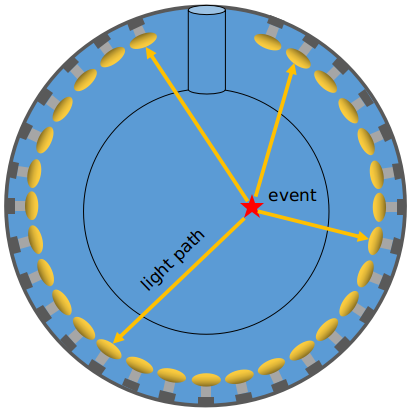
\includegraphics[width=5cm]{mpwDiagram.png}
	\end{minipage}
	\begin{minipage}[t]{0.4\textwidth}
		\centering
		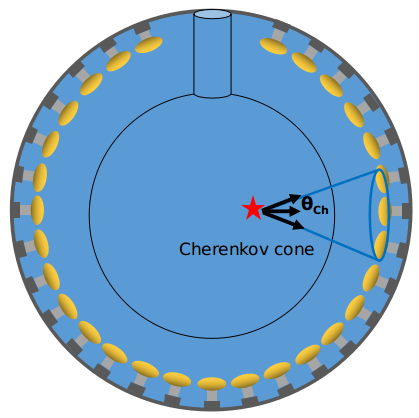
\includegraphics[width=5cm]{mpwDiagram2.png}
	\end{minipage}
	\caption{Diagrams of position (left) and direction (right) reconstruction in SNO+ water phase.}
	\label{mpwdiagram}
\end{figure}


\paragraph{Fitter Structure}

The MPW fitter consists of: 
 Fitter Data : Includes physics constants, set-values and pdfs for the MPW fitter. These parameters are set in the MPW database.
	
	- Water reflection index (water\_RI, or n$_{water}$), used for group velocity ($v_g$ =c/n$_{water}$) calculation. 
	
	The MPW fitter currently uses one fixed number for n$_{water}$, rather than a function of wavelengths. The value of n$_{water}$ can be tuned to give the lowest biases of the fitted positions to the Monte Carlo and to give the lowest RMS of fitted results as well. But the effect of n$_{water}$ can also be corrected by the drive correction afterwards. Currently n$_{water}=1.38486$ is obtained by analyzing the time of flight from the \isotope[16]{N} central run-100934 data reconstructed by the MPW fitter. 
	
	- Constants for fit setting: Includes the fitter tolerance, the maximum iterations for the Multi-path Fitter to converge, time offset, radius cut for position vertex, fitting bin-width and steps.
	
	- Other physics constants: air reflection index (air\_RI), psup radius.
	
	- PMT response time (timing) pdf for the position reconstruction, as shown in \ref{MPW_timingPDF}. The pdf shown in red line is modified from the measured PMT response time distribution from SNO time and the late light response is forced to be de-weighted (black). The pdf is modified in [-100,-4] ns region to match the time residual spectrum obtained from %\isotope[16]{N} central run-100934 (blue).
	
	\begin{figure}[!htb]
		\centering
		%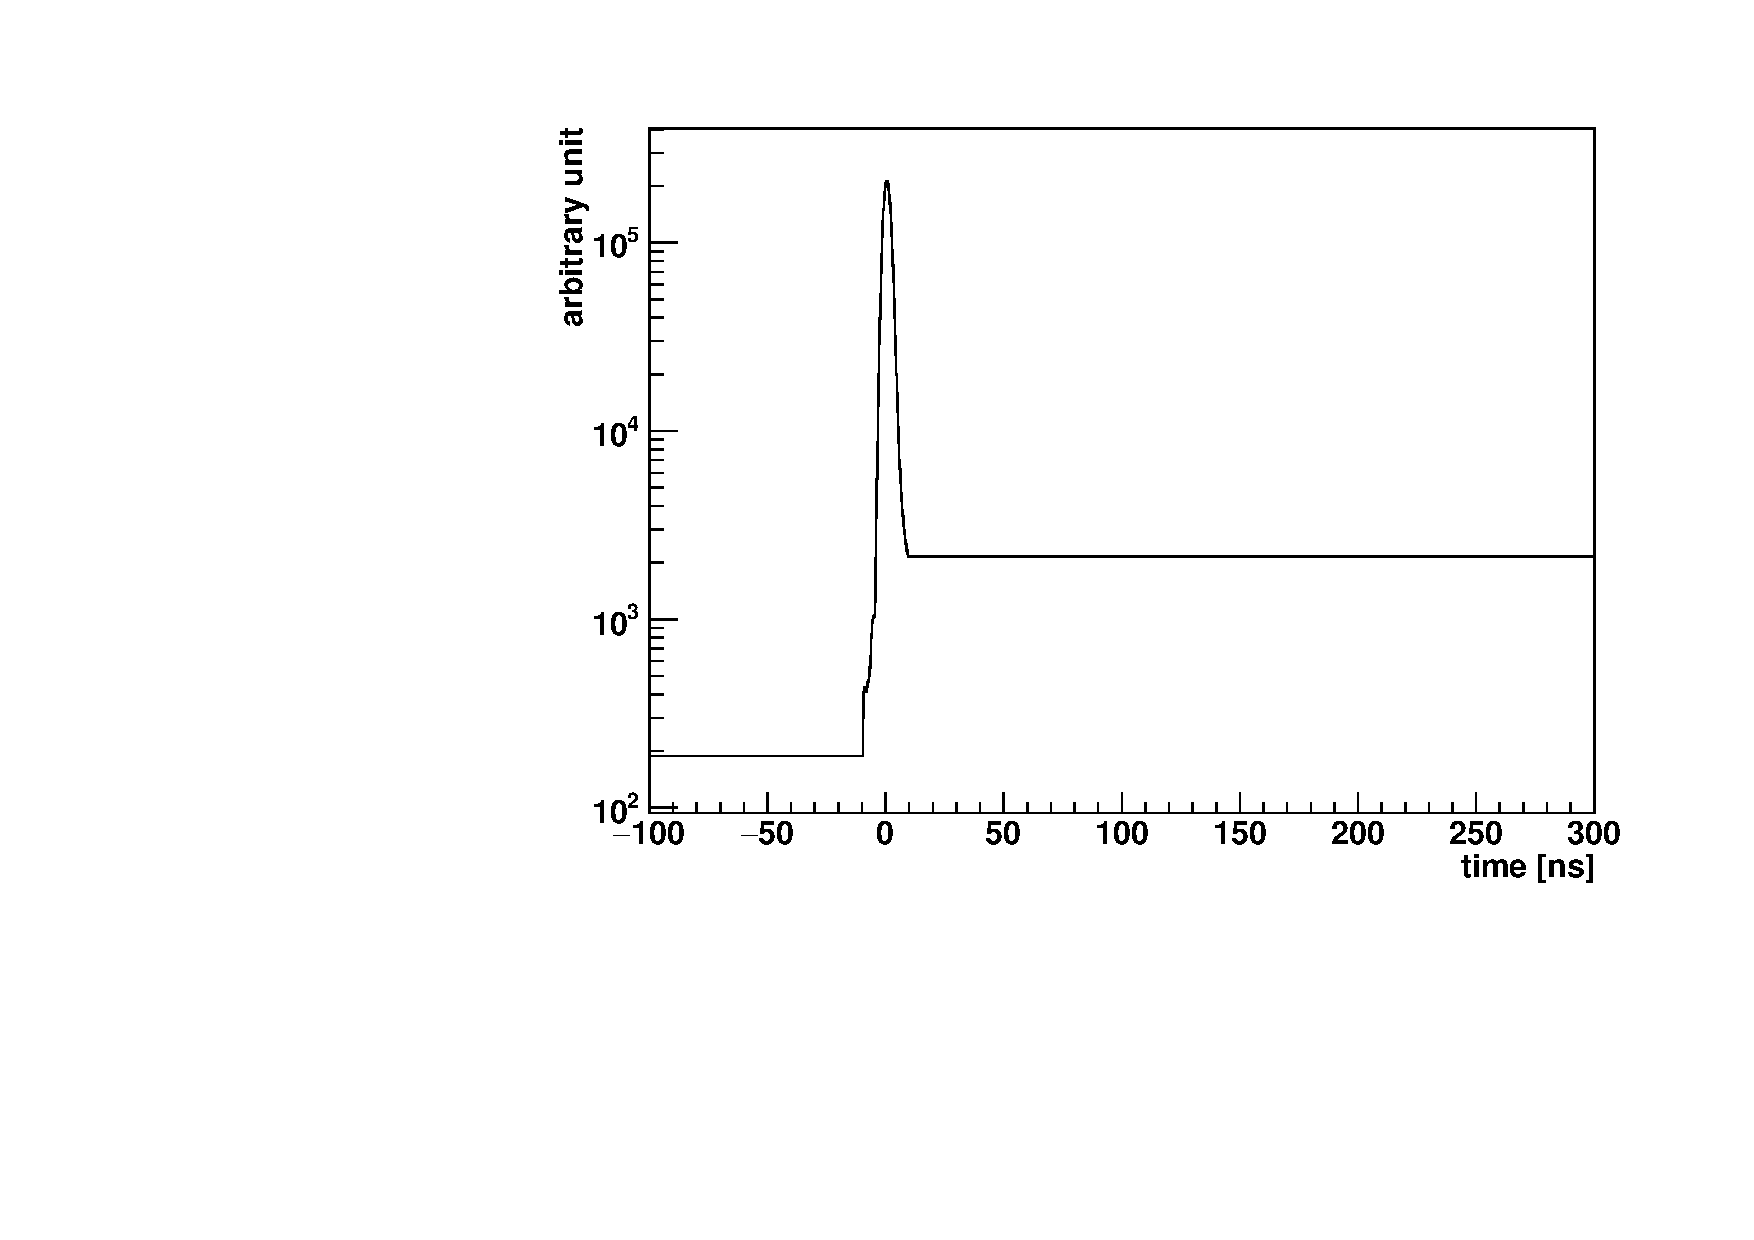
\includegraphics[width=10cm]{recon/MPW_timingPDF.pdf}
		\caption{PMT response time as the timing pdf.}
		\label{MPW_timingPDF}
	\end{figure}
	
	- PMT angular response pdf for the direction reconstruction, as shown in \ref{MPW_angularPDF}. It is taken from the Monte Carlo simulation of 5 MeV electrons traverse in the AV with one direction.
	
	\begin{figure}[!htb]
		\centering
		%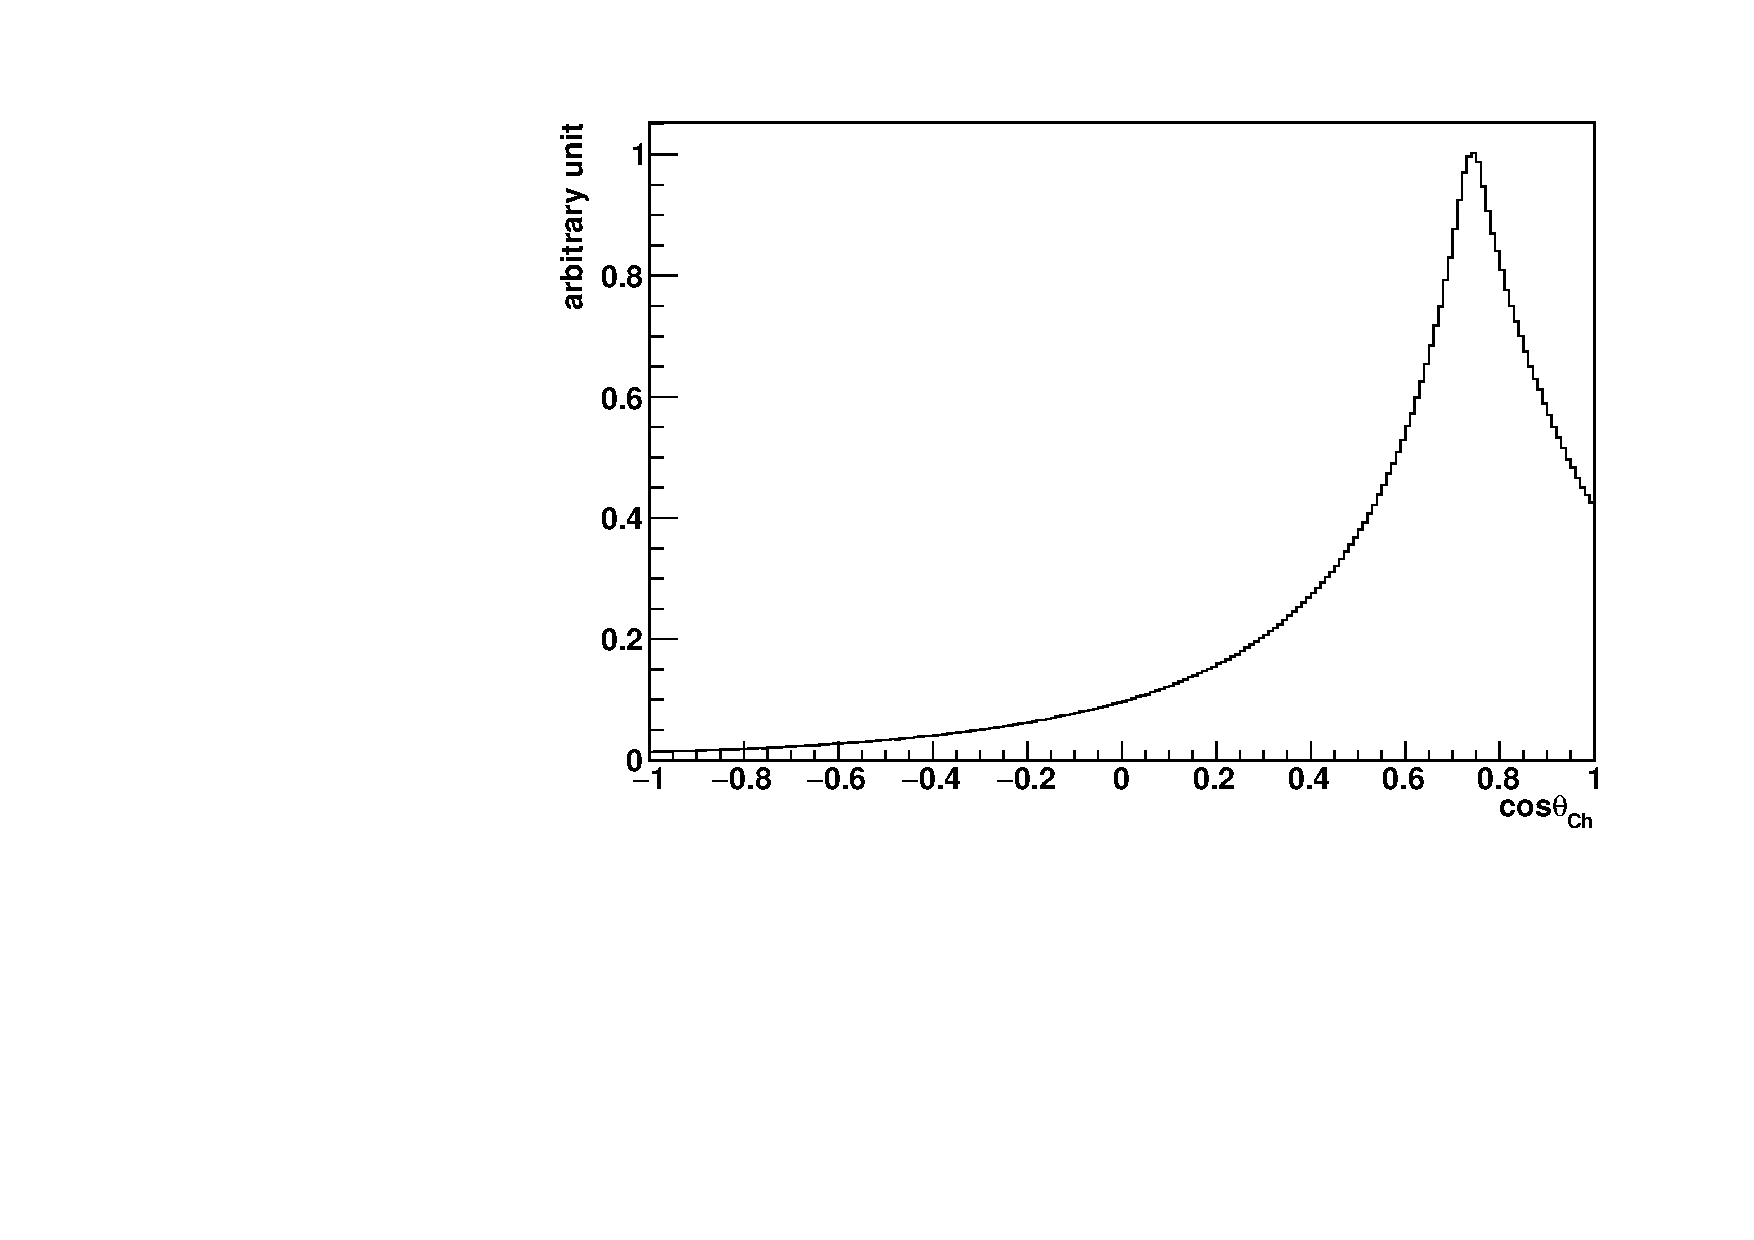
\includegraphics[width=10cm]{recon/MPW_angularPDF.pdf}
		\caption{PMT angular distribution as the angular response pdf.}
		\label{MPW_angularPDF}
	\end{figure}
	
%	\item Fit the position, time and direction.
	
	- Likelihood Calculation Classes: Constructs likelihood functions, calculates likelihoods and their derivatives. For the MPW fitter, there are two classes: WaterPosition for position reconstruction and WaterDirection for direction reconstruction. The WaterPosition class tackles with 4 parameters (x,y,z,t) and the WaterDirection class tackles with 2 parameters ($\theta$,$\phi$). 
	
	- Multi-path Fitter: Processes the MPW fitter and finds the best-fit of the likelihood function. It is a general processor and is shared with the fitters using the Multi-path Fitter, including the MPW fitter, air-water (AW) fitter, wavelength-shifter (WLS) fitter and scint-water fitter (being developed). It processes a certain fitter by being assigned the fitter name in macro. It processes the fitter event by event: for every triggered event, it first calls PMT selectors (ModeCut or StraightTimeResidualCut) and sends the information of the reduced PMTs to a certain Likelihood Calculation Class for likelihood calculations. The Likelihood Calculation Class sends back the values of likelihoods and their derivatives, so the Multi-path Fitter does not care about how the likelihood functions are constructed and how the likelihoods and derivatives are calculated. Using these values, it constructs an n$\times$n Hessian matrix (n is the number of fitting parameters defined in Likelihood Calculation Class) and uses the Levenberg-Marquardt (MRQ) method to maximize the likelihood and finds the best-fit values. For the MPW, if the likelihood maxima is found 5 times for any position and direction then values are returned as the fitted position and direction. For the MPW case, it calls the ModeCut and fitsfor the position and time; then it calls the StraightTimeResidualCut and fits for the directions.
	
	- Dump Likelihood: It is a function inside the Multi-path Fitter. It stores the likelihood surfaces and their derivatives from the fitting of the Multi-path Fitter to check whether the fitter finds global or local maximum of the interested events and to check the reconstruction performances. It requires a switch on/off parameter and the GTIDs of the interested events (a list of GTIDs) from the MPW database.
	
	- SDecompQRH: It is a fit method class modified from ROOT TDecompQRH. It is used by the Multi-path Fitter to invert the Hessian matrix. Compared to ROOT, Solve() for Ax=b is modified to zero the component of x for which the diagonal element in R is small. This allows a Levenberg-Marquardt optimization to continue in many cases
	when the matrix is singular. For the MPW case, it is used to invert 4$\times$4 matrix of the WaterPosition Class while the inversion of 2$\times$2 matrix of the WaterDirection is calculated directly.
	
	- ModeCut: The same class used by Rat. Selects the PMTs of an event by a mode time window. For the MPW, the optimized window is $[-50 + t_{mode}, 100 + t_{mode}]$ ns obtained from %\isotope[16]{N} central run data. 
	
	- StraightTimeResidualCut: Selects the PMTs of an event by a time residue window. This selector requires a fitted position and fitted time. It calculates the time residue directly by assuming straight light path, which is the same method used by Multi-path fitter. For the MPW case, it is used for the direction fit after the position and time are reconstructed. The default window is [-10, 250] ns.

\section{MPW Position and Direction Reconstructions}


\subsection{Vertex Reconstruction}
For the position reconstruction of the MPW fitter, the likelihood function simply calculates the likelihood assuming straight line paths of prompt light from a position vertex $\vec{X_0}$ ($\mathrm{fVertex}$) and a starting time offset $t_0$ to each of the hit PMTs. 

We define the position difference $\vec{X}_{{\mathrm{diffCh}}} = \vec{X_0}-\vec{X}_{\mathrm{pmt}}$, then the time of flight for prompt light is  $t_{\mathrm{Ch}}=|\vec{X}_{{\mathrm{diffCh}}}|/v_g$ and $L_{\mathrm{Ch}}=L(t_{\mathrm{Ch}})$.

The derivatives of the likelihood function can be calculated from explicit mathematical forms as:
\[
\frac{\partial L}{\partial t_0}=\frac{dL_{\mathrm{Ch}}}{dt_{\mathrm{Ch}}},
\]

\[
\frac{\partial L}{\partial x}=\frac{\partial L_{\mathrm{Ch}}}{\partial t_{\mathrm{Ch}}}\frac{dt_{\mathrm{Ch}}}{\partial x}=-\frac{dL_{\mathrm{Ch}}}{dt_{\mathrm{Ch}}}\frac{X_{{\mathrm{diffCh}}}}{|\vec{X}_{{\mathrm{diffCh}}}|\cdot v_g},
\]

\[
\frac{\partial L}{\partial y}=-\frac{dL_{\mathrm{Ch}}}{dt_{\mathrm{Ch}}}\frac{Y_{{\mathrm{diffCh}}}}{|\vec{X}_{{\mathrm{diffCh}}}|\cdot v_g},
\]

\[
\frac{\partial L}{\partial z}=-\frac{dL_{\mathrm{Ch}}}{dt_{\mathrm{Ch}}}\frac{Z_{{\mathrm{diffCh}}}}{|\vec{X}_{{\mathrm{diffCh}}}|\cdot v_g},
\]

where $\frac{dL_{\mathrm{Ch}}}{dt_{\mathrm{Ch}}}$ can be calculated numerically from the timing pdf. 

In the WaterPosition class, it starts with a random ($\vec{x}_0,t_0$) as seed and calculates the likelihoods and their derivatives for various paths. These values are sent to the Multi-path Fitter, which is fitting 4 parameters: $x,y,z,t$ and to maximize the likelihood function through the MRQ method and to find the best-fit positions.

\subsection{Direction Reconstruction}
 $\vec{u}_{0}=(\cos\phi\sin\theta,\sin\phi\sin\theta,\cos\theta)$ ($\mathrm{fDirection}$), where the $\theta$ is zenith angle and $\phi$ the azimuth. $\cos\theta_{\mathrm{Ch}}$ is the angle between $\vec{u}_{0}$ and $\vec{X}_{{\mathrm{diffCh}}}$, which is taken as the fitting parameter of the likelihood function for the direction reconstruction. For the i-th hit PMT, $\cos\theta^i_{\mathrm{Ch}}=\vec{u}_0\cdot\frac{\vec{X}^i_{{\mathrm{diffCh}}}}{|\vec{X}^i_{{\mathrm{diffCh}}}|}$, then the likelihood function is:
\[
L(\vec{u}_0)=\sum_{i=1}^{{\mathrm{Nhits}}}L_i(\cos\theta_{\mathrm{Ch}}^i),
\]

The derivatives have explicit mathematical forms:
\[
\frac{\partial L}{\partial\theta}=\frac{dL_{\mathrm{Ch}}}{d\cos\theta_{\mathrm{Ch}}}\frac{d\cos\theta_{\mathrm{Ch}}}{\partial\theta}
=\frac{dL_{\mathrm{Ch}}}{d\cos\theta_{\mathrm{Ch}}}\frac{d\vec{u}_0}{d\theta}\cdot\frac{\vec{X}_{{\mathrm{diffCh}}}}{|\vec{X}_{{\mathrm{diffCh}}}|},
\]
where $d\vec{u}_0/d\theta=(\cos\phi\cos\theta, \sin\phi\cos\theta, -\sin\theta)$ and 
\[
\frac{\partial L}{\partial\phi}=\frac{dL_{\mathrm{Ch}}}{d\cos\theta_{\mathrm{Ch}}}\frac{d\cos\theta_{\mathrm{Ch}}}{d\phi}
=\frac{dL_{\mathrm{Ch}}}{d\cos\theta_{\mathrm{Ch}}}\frac{d\vec{u}_0}{d\phi}\cdot\frac{\vec{X}_{{\mathrm{diffCh}}}}{|\vec{X}_{{\mathrm{diffCh}}}|},
\] where $d\vec{u}_0/d\phi=(-\sin\phi\sin\theta, \cos\phi\sin\theta, 0)$. $\frac{dL_{\mathrm{Ch}}}{d\cos\theta_{\mathrm{Ch}}}$ can be calculated numerically from the PMT angular response pdf.

In the FitterWaterDirection class, it starts with a random ($\theta_0,\phi_0$) as seed and calculates the likelihoods and their derivatives for various paths. These values are sent to the Multi-path Fitter, which is now fitting 2 parameters: ($\theta,\phi$) and to maximize the likelihood function through the MRQ method and to find the best-fit directions.

\subsection{Drive Correction}

An effect of `fitter pull' in the event vertex reconstruction utilizing the Cherenkov light was observed in the SNO experiment. The cause of this effect is that the Cherenkov photons trigger the majority of PMT hits with early timing and these hits are located within the Cherenkov cone; while the scattered or reflected light with later timing trigger PMT hits throughout the detector. This 



%\begin{figure}[!htb]
%	\centering
%	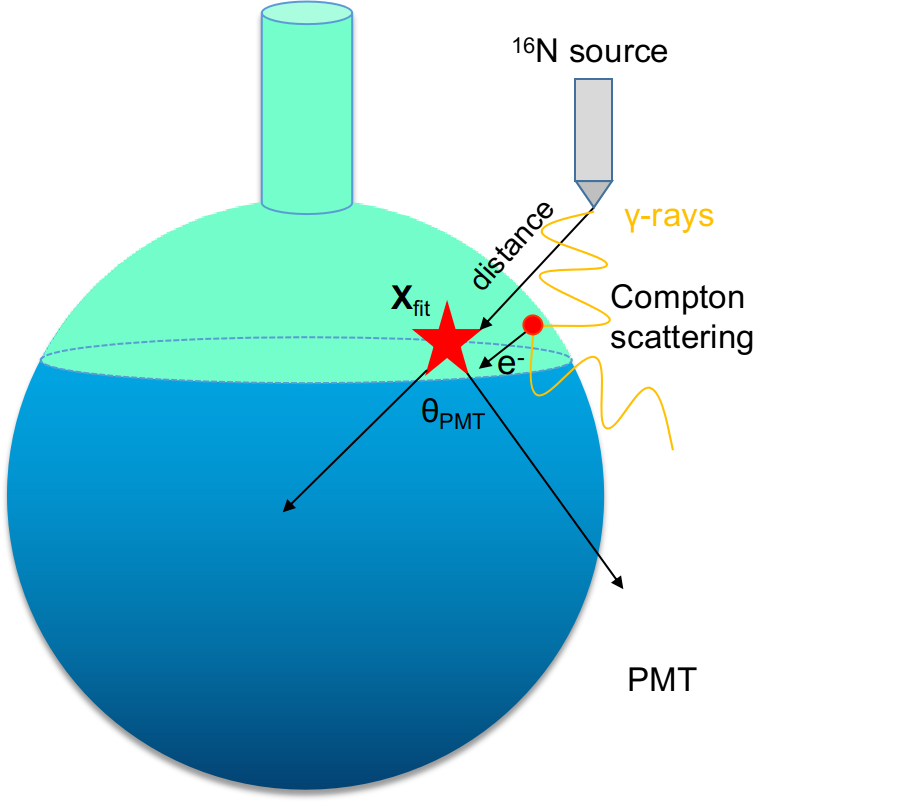
\includegraphics[width=6cm]{partialN16.png}
%\caption{ modified from Fig.~C.2 in \cite{brice1996monte}.}
%	\label{drivecor}
%\end{figure}

 as illustrated in Fig. .

  
 

shift 

fitter pull.



\cite{brice1996monte,coulter2013modelling}.


Once the MPW fitter obtains the fitted position and direction, a drive correction is applied on the fitted position by $\vec{X}_{\mathrm{corrected}} = p_0\vec{X}_{fit}+p_1\vec{u}_{fit}$, where $p_0$ and $p_1$ are the correction parameters.


To obtain the values of $p_0$ and $p_1$, we generated electron events distributed isotropically inside the AV. The simulations of 2, 3, 4, ... ,10 MeV electrons are produced. Then the MPW fitter is applied on each simulations and returns the results of $\vec{X}_{fit}$ and $\vec{u}_{fit}$. Take the Monte Carlo generated positions $\vec{X}_{MC}$ as the true positions, for all the fitted events, a $\chi^2$ function is calculated by:
\[
\chi^2 = \sum_{i=1}^{N_{\mathrm{events}}}[\vec{X}^i_{MC}-(p_0\vec{X}^i_{fit}+p_1\vec{u}^i_{fit})]^2
\]

The $p_0$ and $p_1$ are obtained by minimizing the $\chi^2$ function. 
When doing the $\chi^2$ calculation, the fitted events of $|\vec{X}_{fit}-\vec{X}_{MC}|>3~m$ are thrown away to improve the $\chi^2$ minimization results.

For the 2 to 10 MeV electrons simulations, the obtained values of $p_0$ and $p_1$ are energy or Nhit dependent. However, it does not improve the results if using the Nhit dependent functions $p_0(Nhit)$ and $p_1(Nhit)$ as drive corrections.
Finally we take the average values from the 5 to 10 MeV electrons simulations and the drive correction is set as $\vec{X}_{\mathrm{corrected}} = 0.995765\vec{X}_{fit}+-63.826\vec{u}_{fit}$.

It is important to note that since the drive correction parameters are obtained from the reconstructions of Monte Carlo, it depends on the Monte Carlo and the results of reconstruction. Therefore, the n$_{water}$, mode cut and time residue cut affecting the fitted results will also affect the drive correction parameters, but not significantly.

By fitting the simulations of 5 MeV electrons generated at the detector center and travelling along +X direction, the drive effct of the MPW fitter causes a $\sim$50 mm biases from the detector center along +X axis. The drive correction reduces this drive bias down to $\sim$0.2 mm. For the reconstruction of \isotope[16]{N} data, the drive correction can reduce the fitted position RMS by $\sim$20 mm.





\section{Vertex and Direction Reconstruction for Wavelength-shifter}




\section{Vertex Reconstruction for Partial-fill and Scintillator Phases}

In the partial fill geometry, photons will travel with different speeds as they pass through two different mediums, water and scintillator. Assuming a straight light path, the MP Partial Fitter mainly calculates the total length of the light path ($|\vec{l}_p|=|\vec{X}_\mathrm{PMT}-\vec{X}_0|$) and separates it into the lengths in scintillator ($d_{sp}$) and in water ($|\vec{l}_p|-d_{sp}$).

\begin{figure}[!htb]
	\centering
	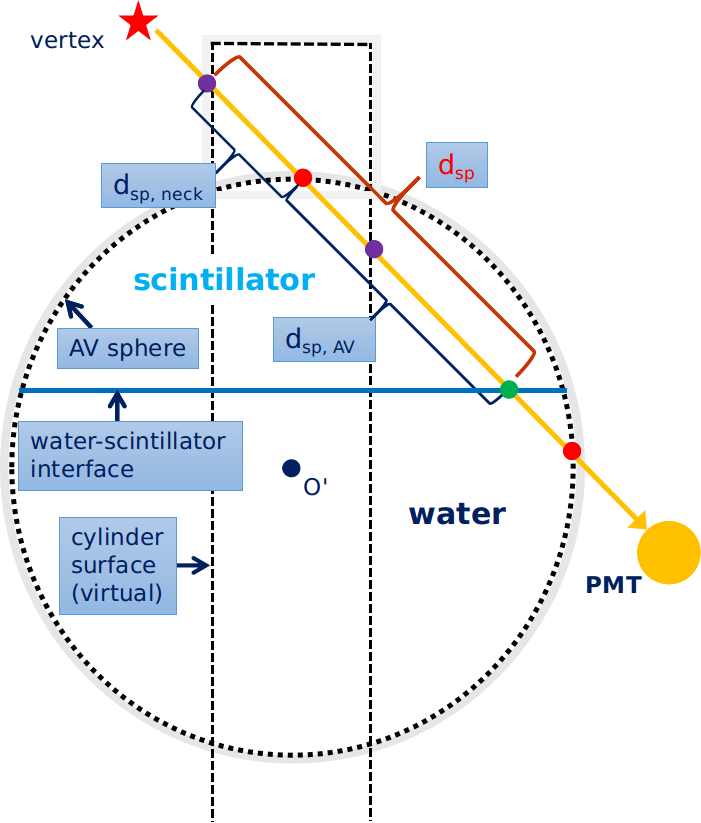
\includegraphics[width=7cm]{scintpath.png}
	\caption{Light path calculation for the MP Partial Fitter.}
	\label{scintpath}
\end{figure}

As illustrated in Figure~\ref{scintpath}, a detailed calculation of $d_{sp}$ includes evaluations of (1) light path and neck (line-cylinder) intersection; (2) light path and AV sphere (line-sphere) intersection and (3) light path and water-scintillator interface (line-plane) intersection. $d_{sp}$ is further separated into the path length in neck ($d_{sp,neck}$) and in AV ($d_{sp,AV}$).

Then the time of flight is obtained by:
\begin{equation}
tof = \frac{|\vec{l}_p|-d_{sp}}{v_{gr,water}} +\frac{d_{sp}}{v_{gr,scint}},
\end{equation}
The time residual is $t_{res} = t_\mathrm{PMT}-tof-t_0$.

\begin{figure}[htbp]
	\centering	
	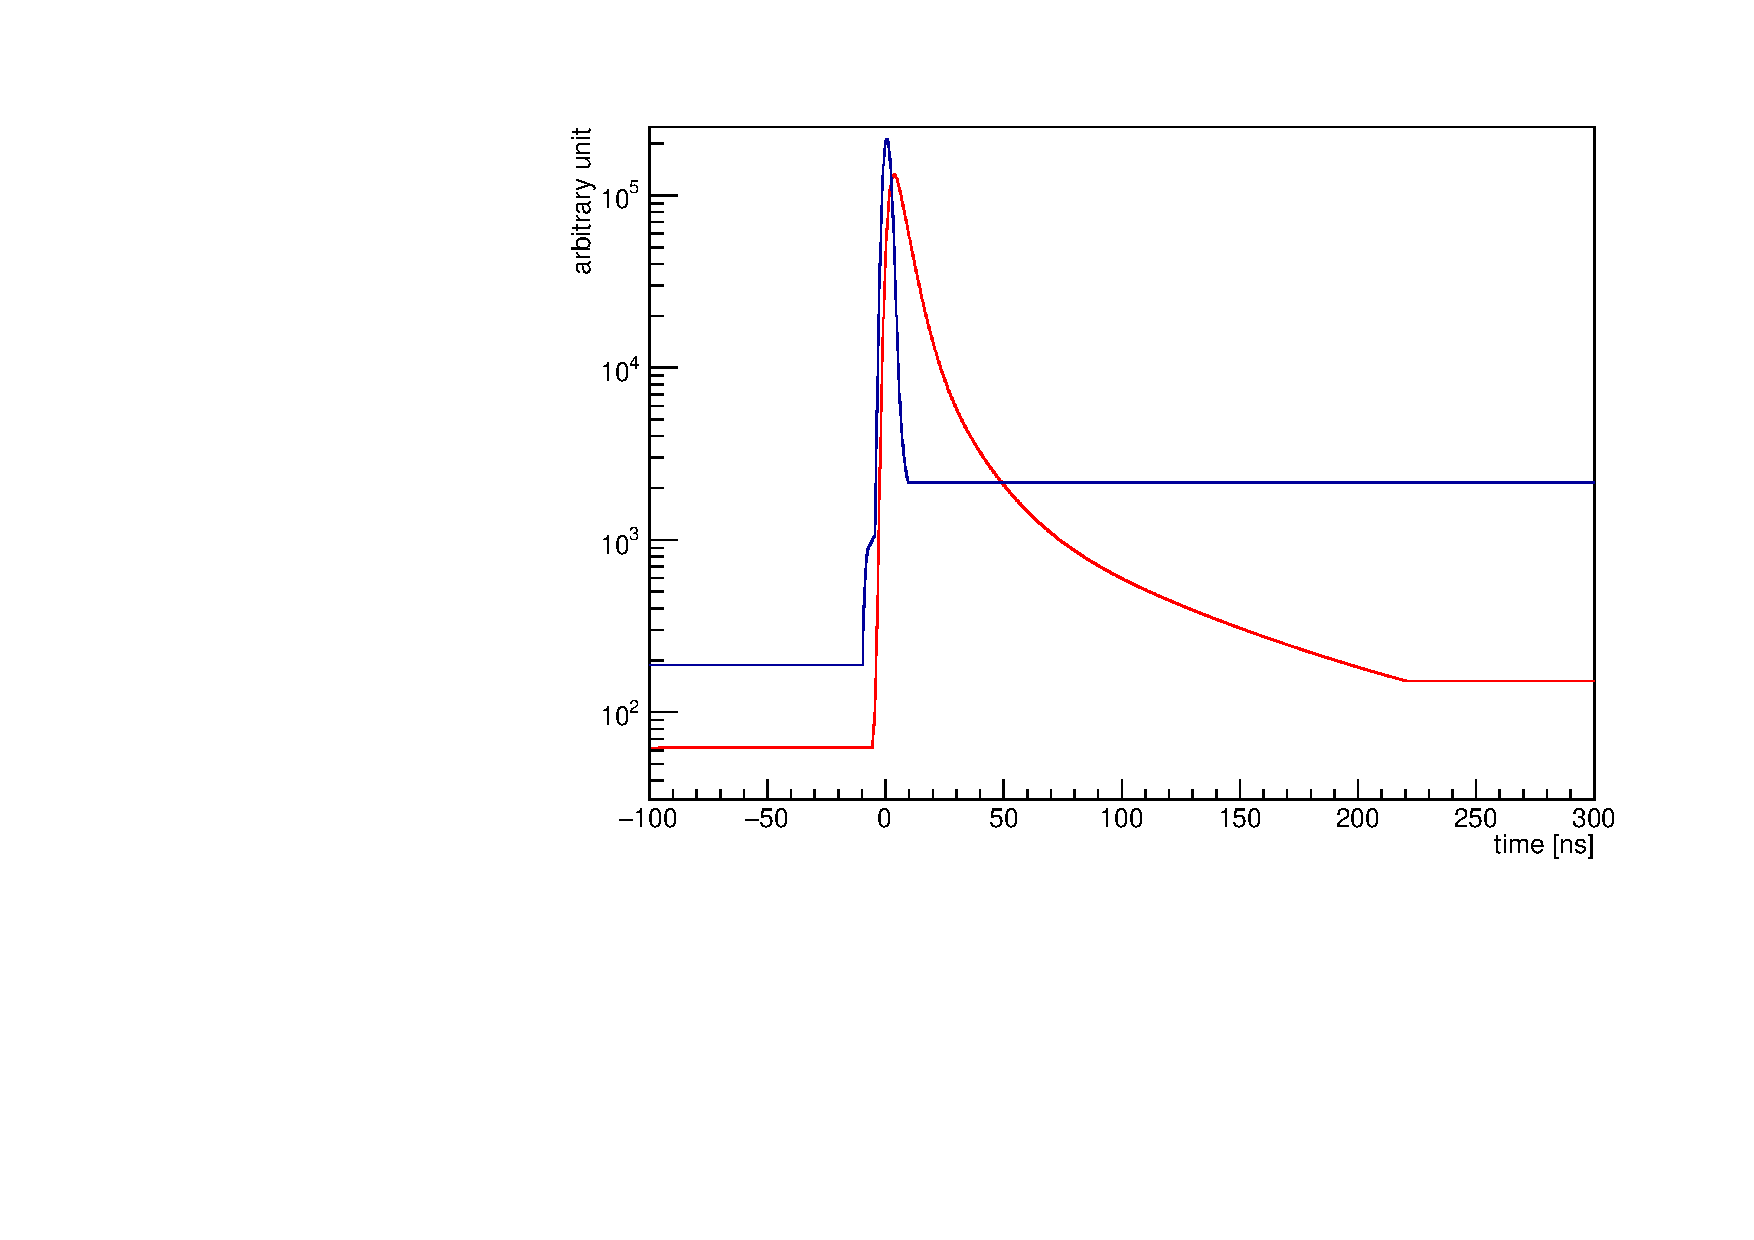
\includegraphics[width=7cm]{scintpdf.pdf}
	\caption{The timing pdfs used by the MP Partial Fitter. Blue: the timing pdf used by the MP Water Fitter; Red: the scintillator timing pdf.}
	\label{partialpdf}
\end{figure}

If $d_{sp}=0$, the light path is always in the water. In this case, the fitter is the same as the MP Water Fitter. The fitter fits with the MP Water Fitter pdf. Once the light path passes through the scintillator region, the fitter fits with a scintillator timing pdf, the PMT time response modified to photon propagation time in scintillator, as shown in Figure~\ref{partialpdf}.

\begin{figure}[htbp]
	\centering
	\subfigure[scintillator region]{
		\begin{minipage}[t]{0.38\textwidth}
			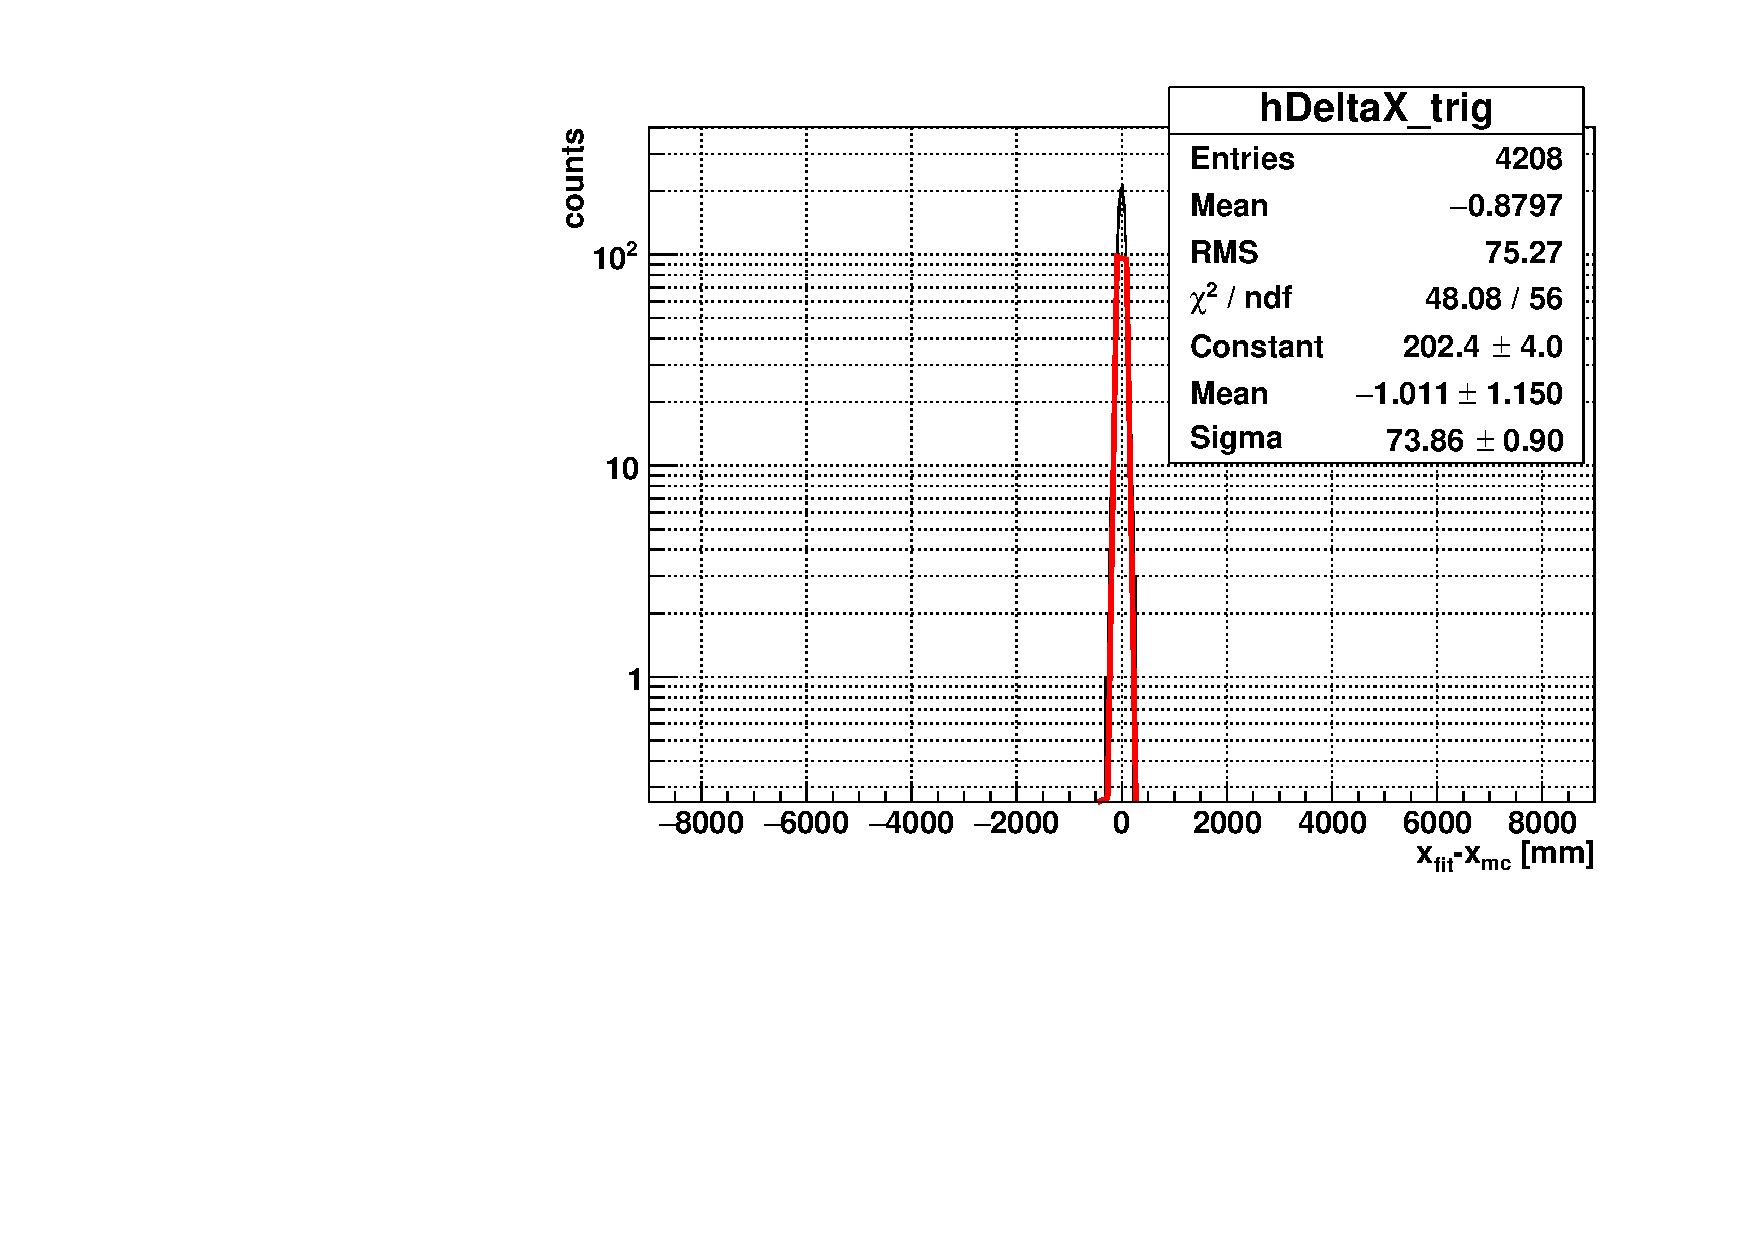
\includegraphics[width=6cm]{partial_top_x.pdf}
		\end{minipage}
	}   
\subfigure[water region]{ 
		\begin{minipage}[t]{0.38\textwidth}
			\centering
			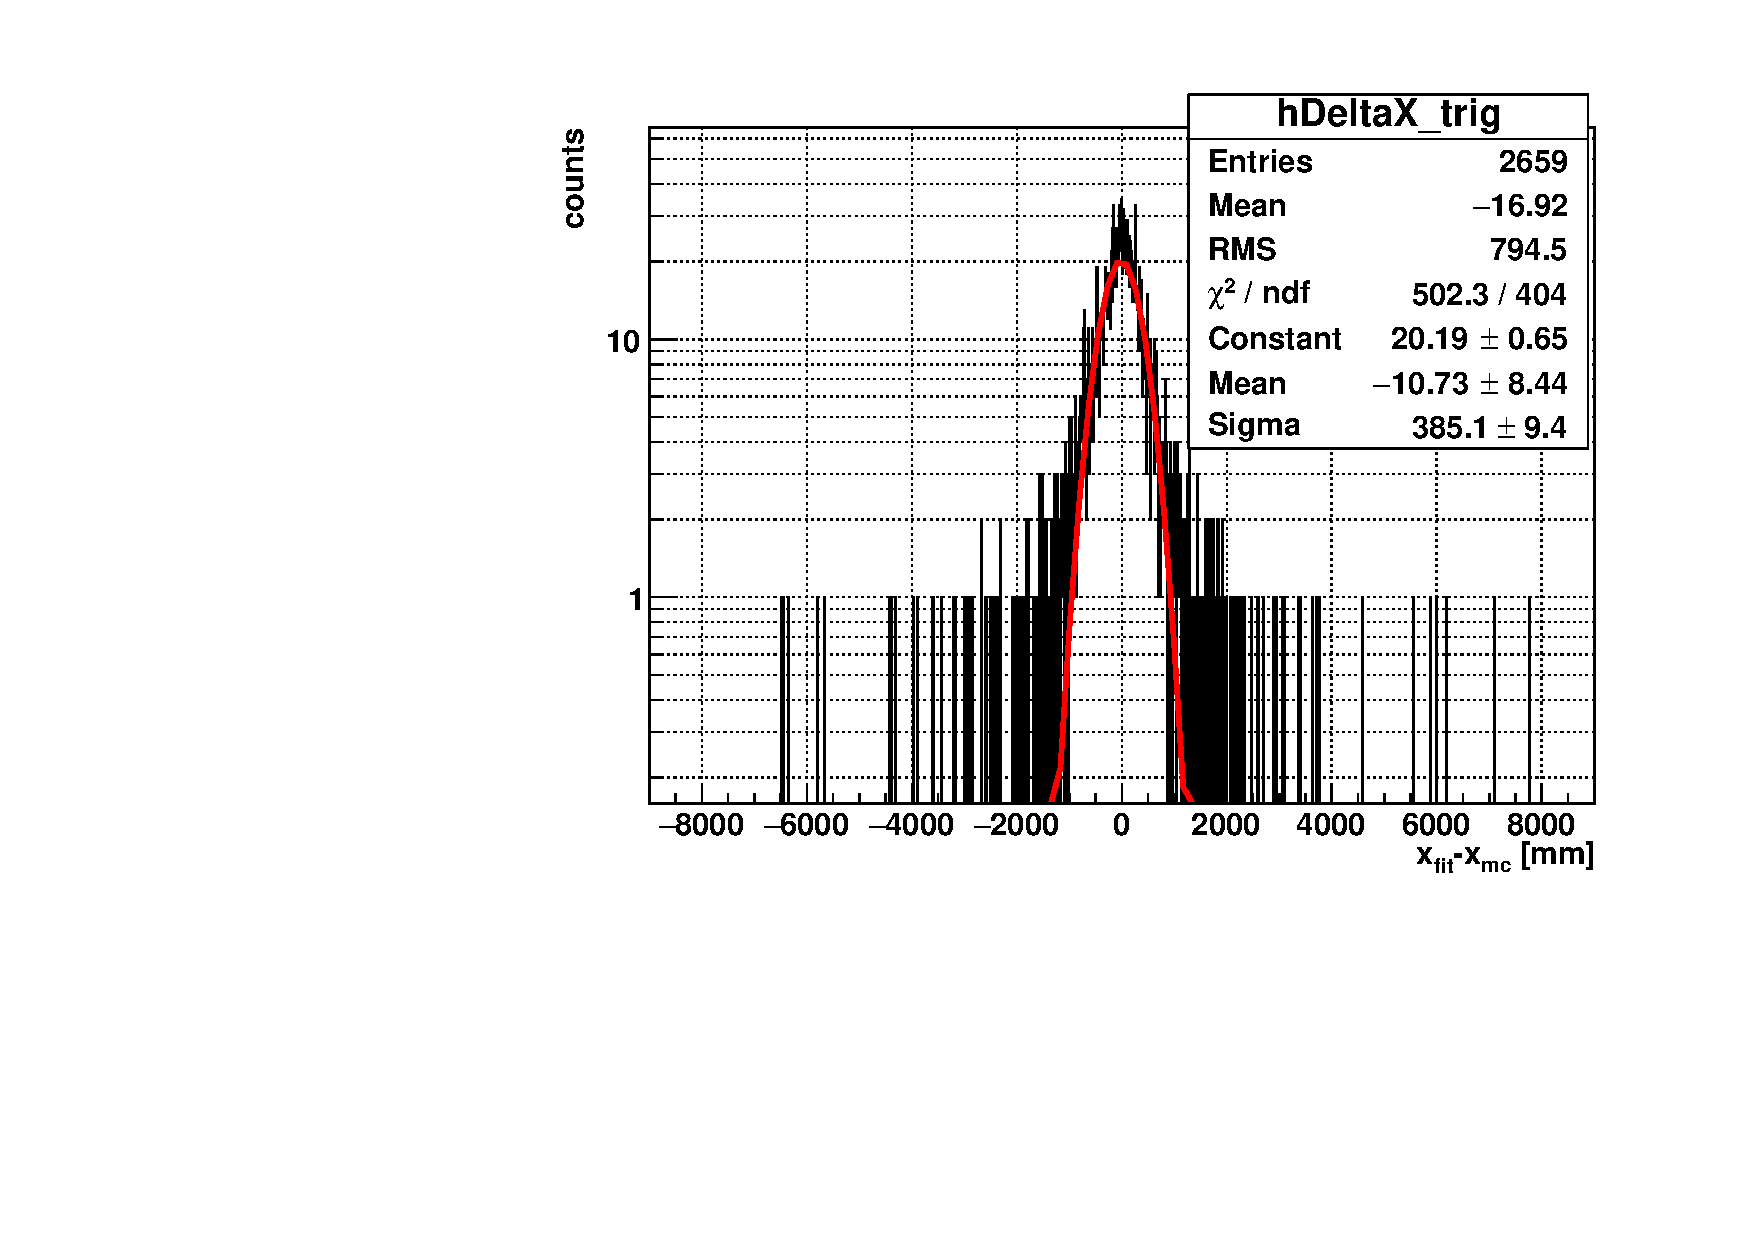
\includegraphics[width=6cm]{partial_bot_x.pdf}
		\end{minipage}
	}
	\subfigure[whole region]{ 
		\begin{minipage}[b]{0.32\textwidth}
			\centering
			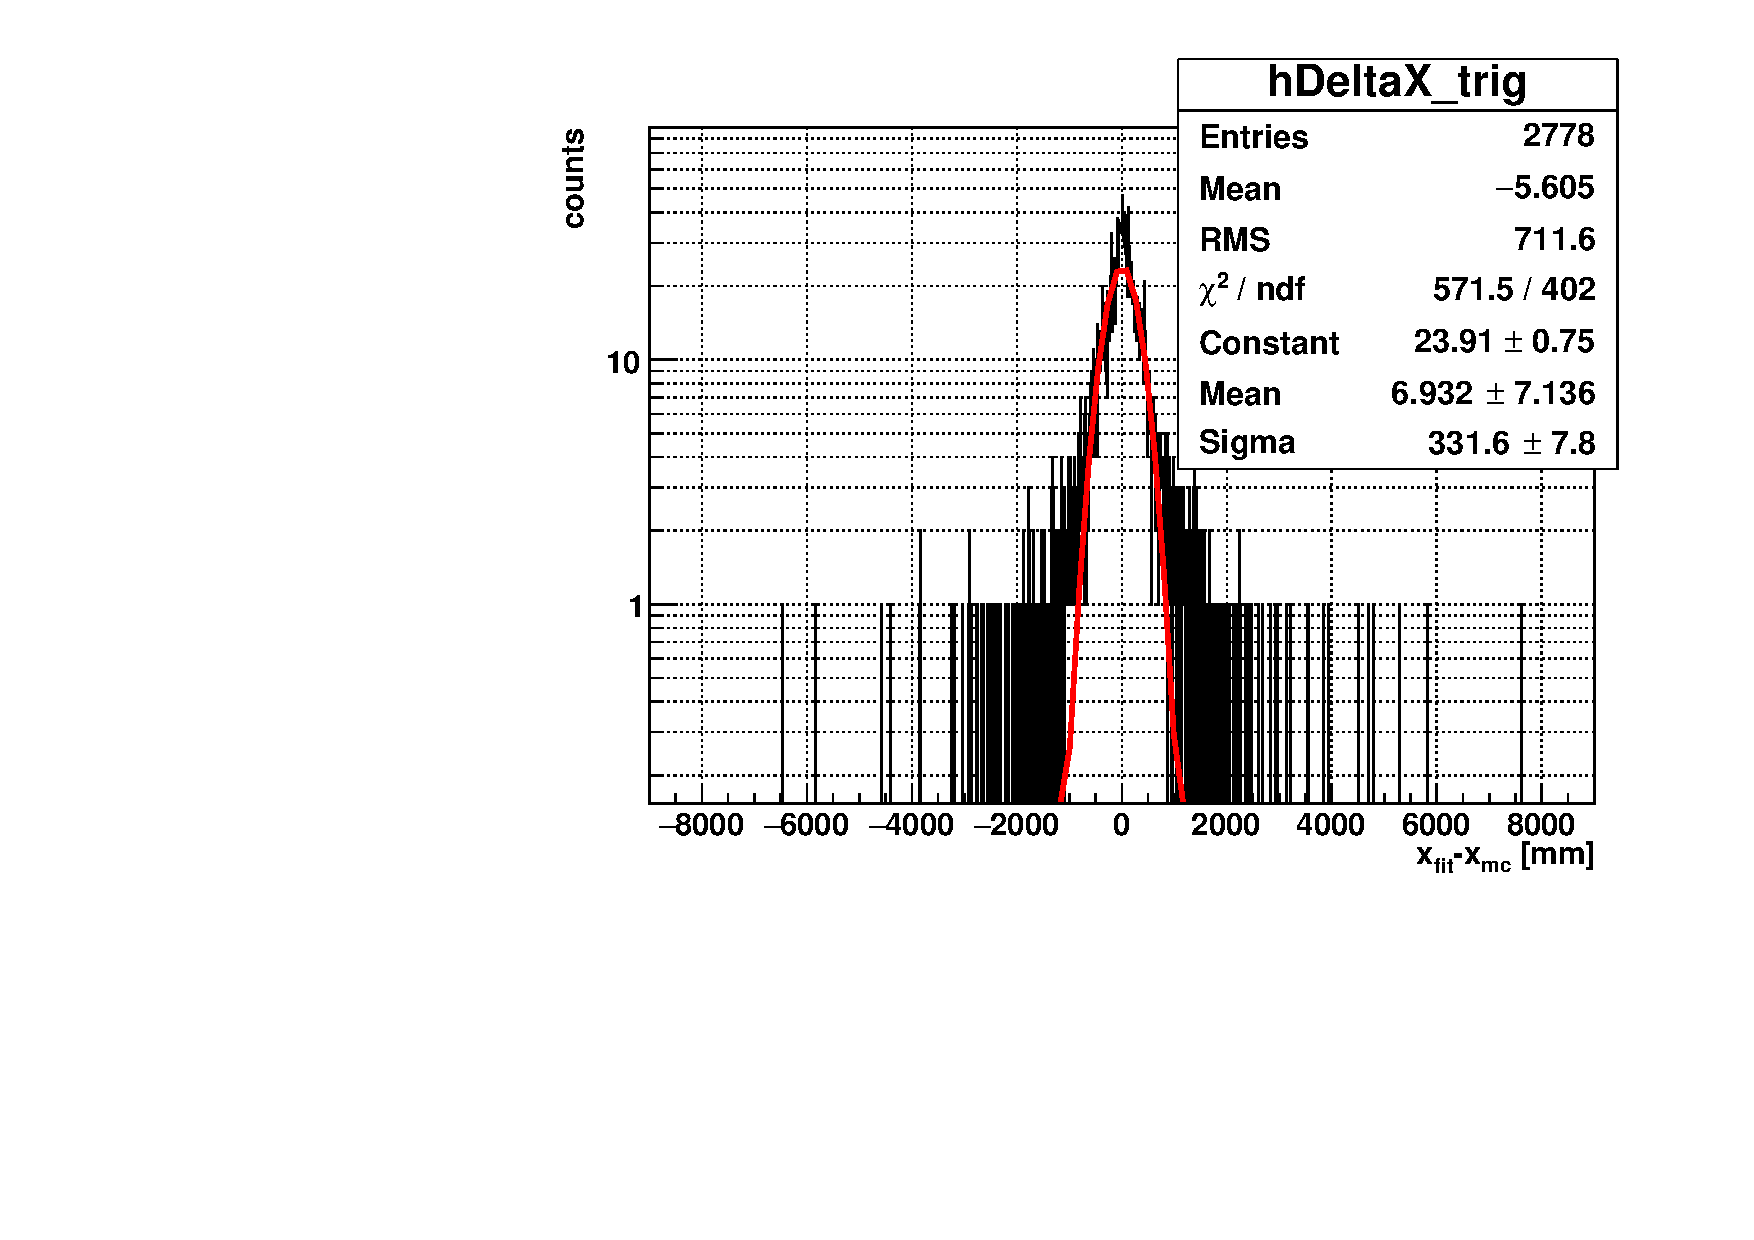
\includegraphics[width=6cm]{partial_full_x.pdf}
		\end{minipage}
	}
	\caption{Distributions of fit position bias projected on x axis ($x_{fit}-x_{MC}$).}
	\label{partial_fit_x}
	\subfigure[scintillator region]{ 
		\begin{minipage}[t]{0.38\textwidth}
			\centering
			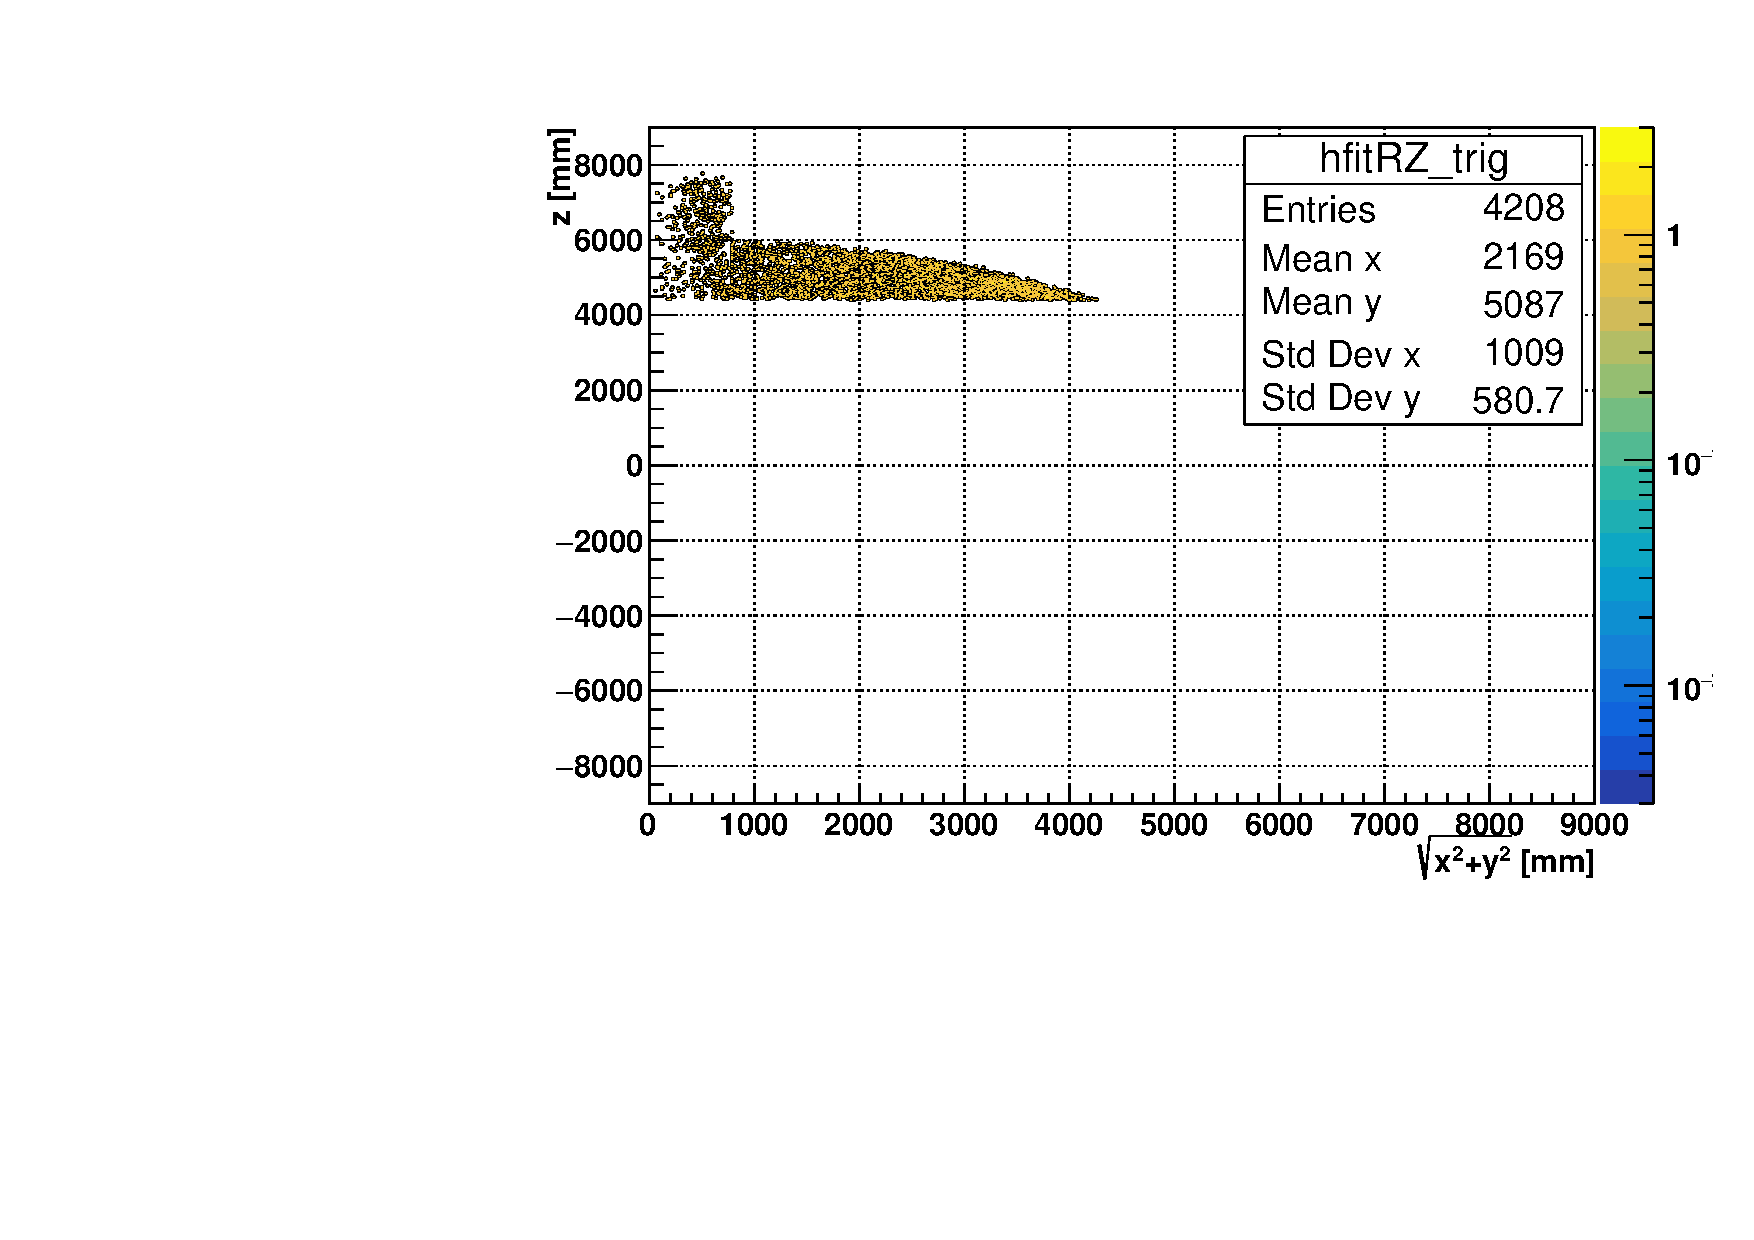
\includegraphics[width=5.8cm]{partial_top_r.pdf}
		\end{minipage}
	}
	\subfigure[water region]{ 
		\begin{minipage}[t]{0.38\textwidth}
			\centering
			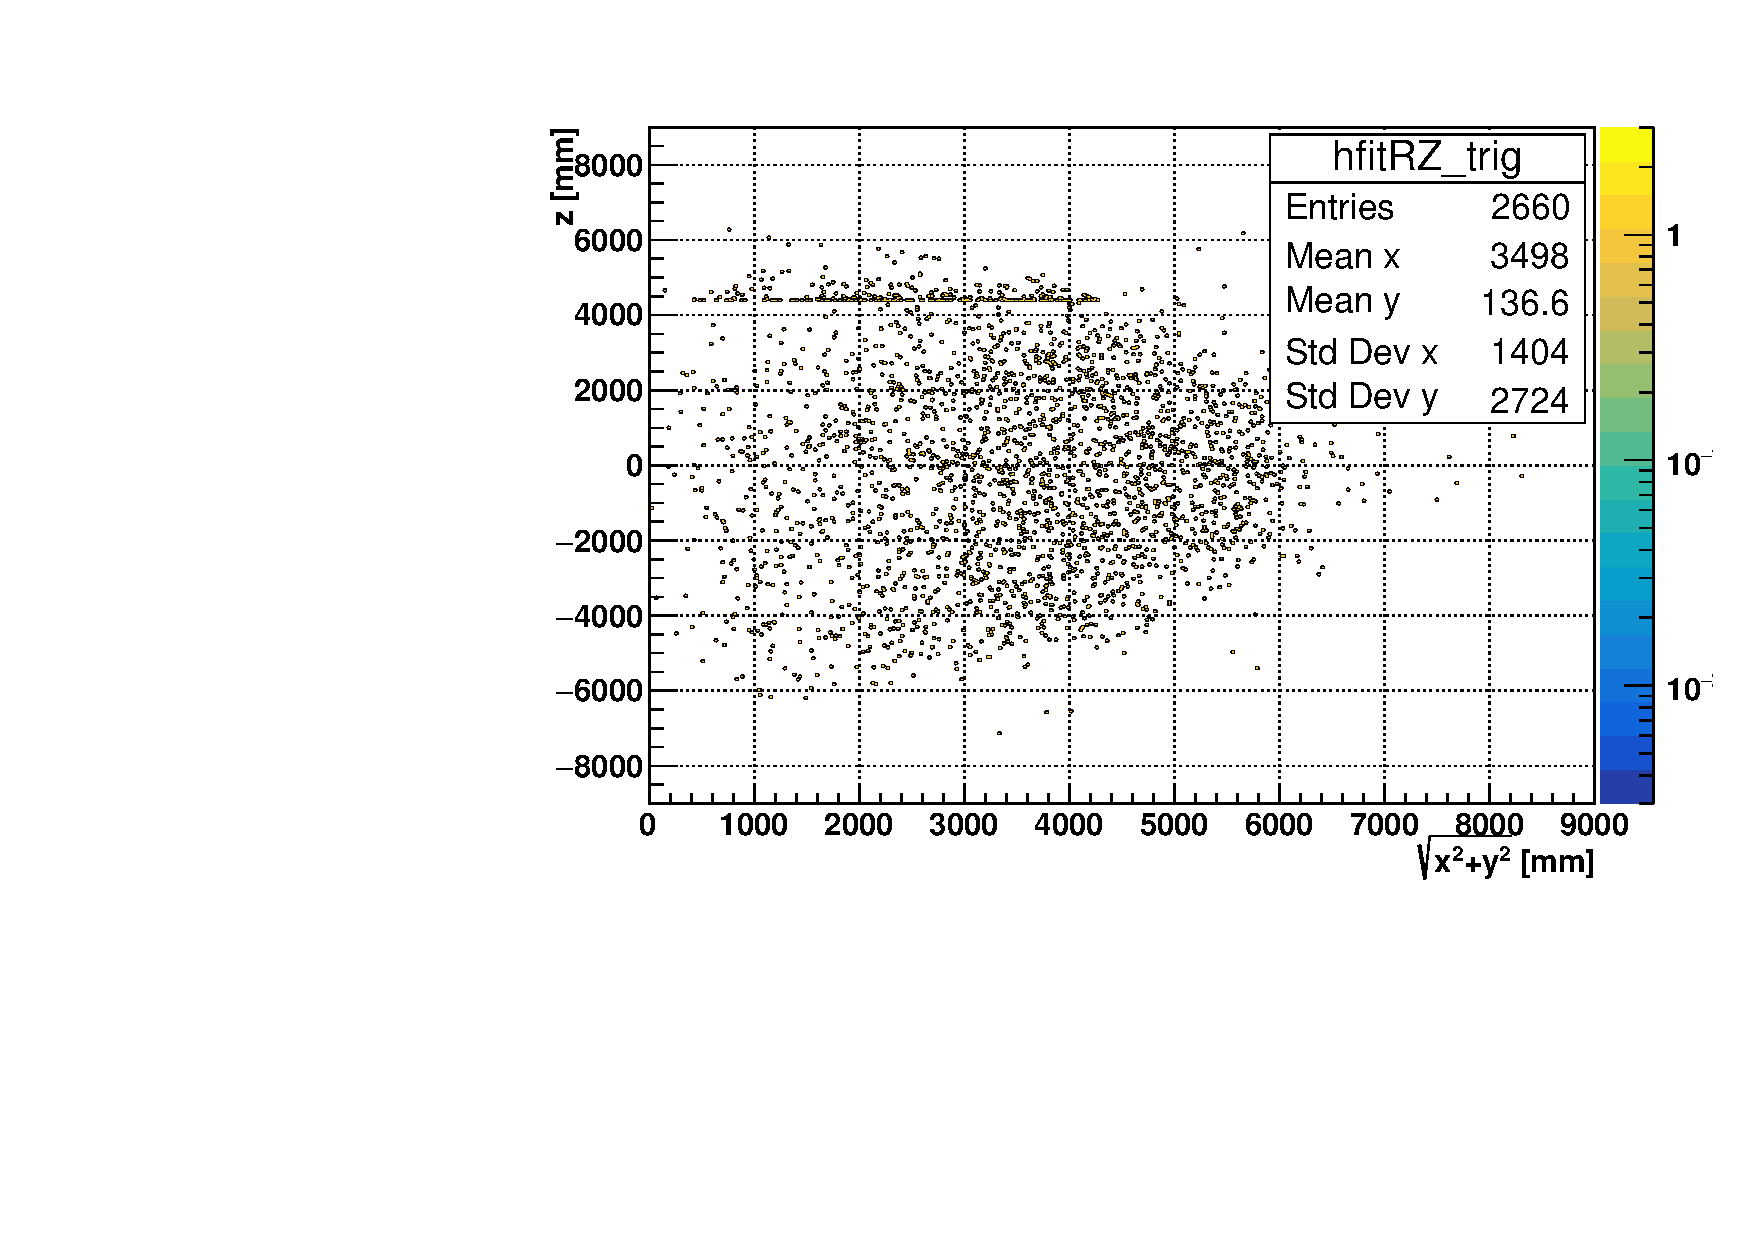
\includegraphics[width=5.8cm]{partial_bot_r.pdf}
		\end{minipage}
	}
	\subfigure[whole region]{ 
		\begin{minipage}[b]{0.35\textwidth}
			\centering
			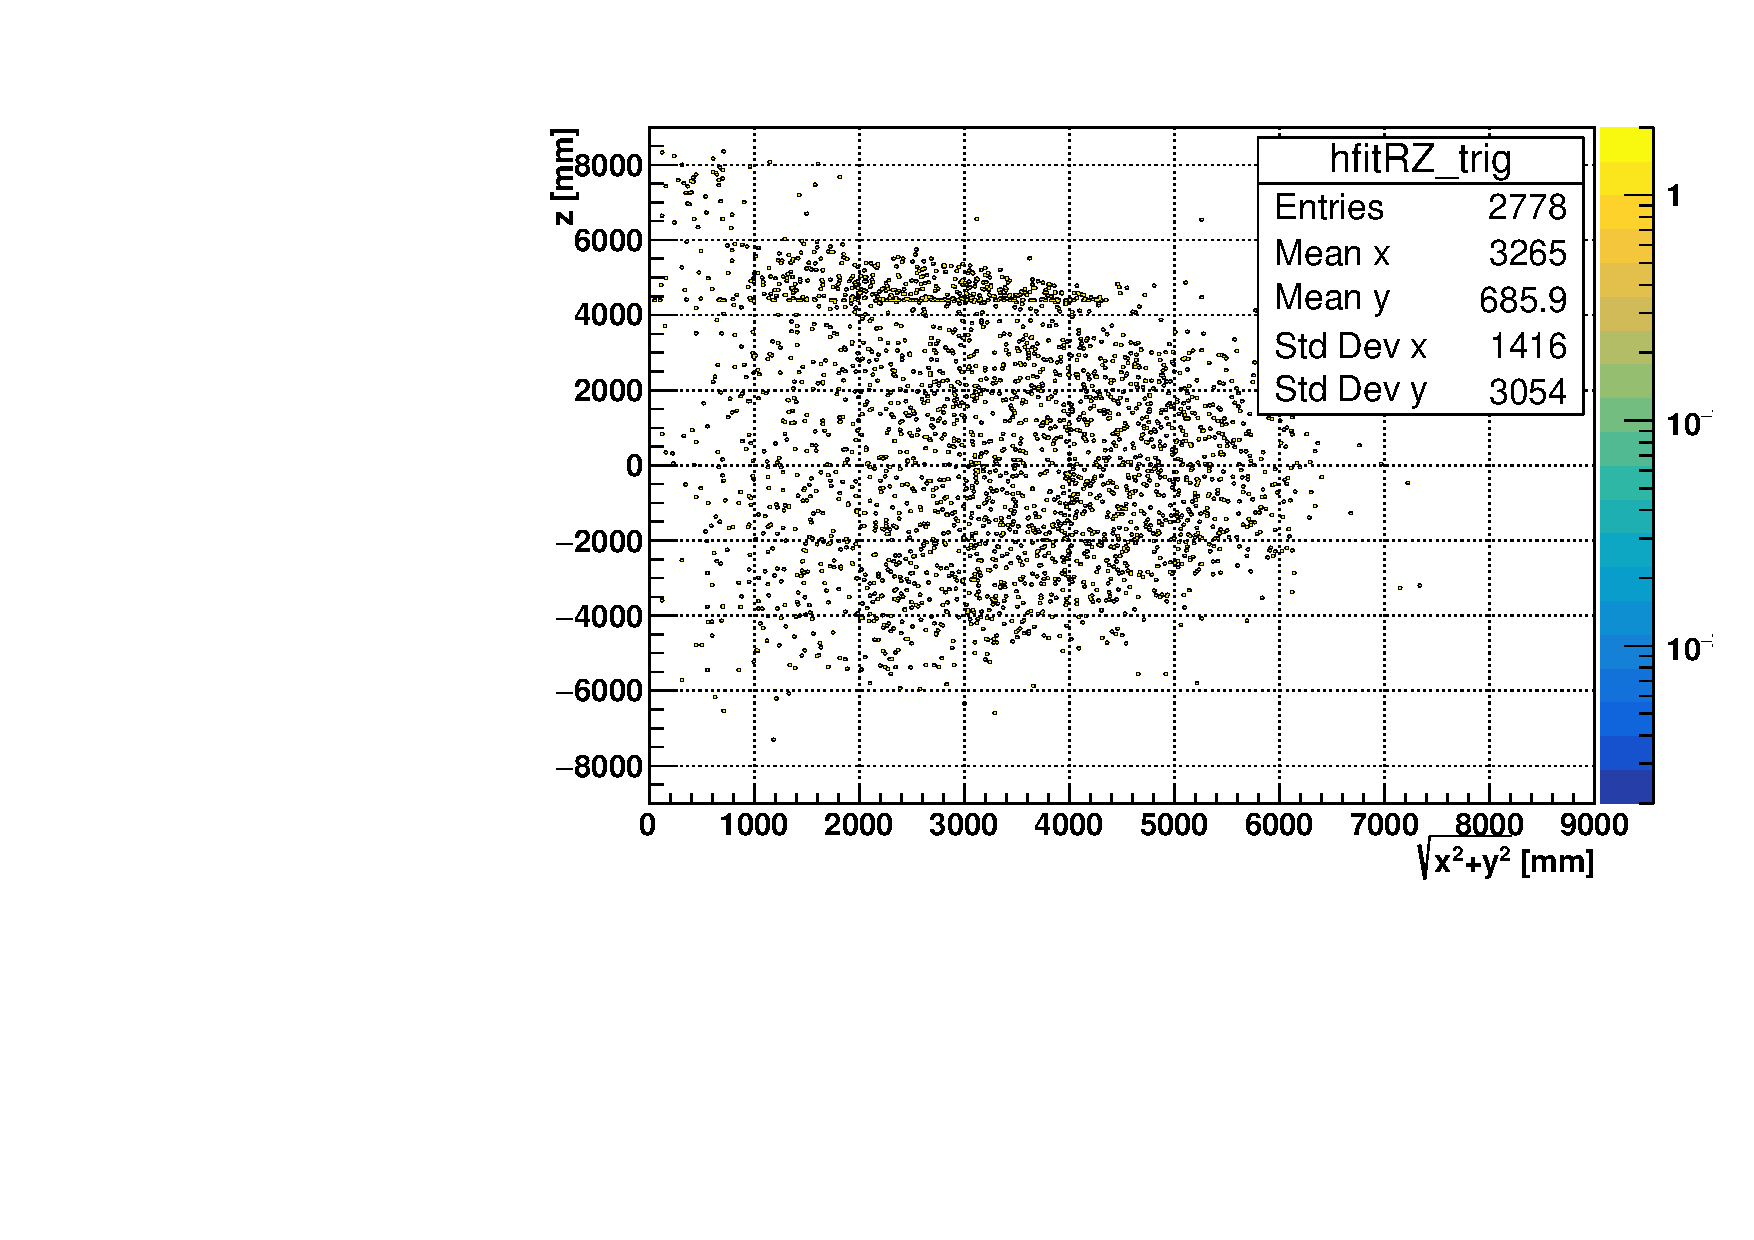
\includegraphics[width=5.8cm]{partial_full_r.pdf}
		\end{minipage}
	}
	\caption{Fit results: $\rho_{fit}=\sqrt{x_{fit}^2+y_{fit}^2}$ vs. $z_{fit}$.}
	\label{partial_fit_rz}
\end{figure}

The performance of the fitter was studied with MC simulations. In a partial fill geometry with water level at 4.4 m, 2.5 MeV electrons are simulated inside the AV in the scintillator region only, the water region only and the whole AV region.

Figure~\ref{partial_fit_x} and Figure~\ref{partial_fit_rz} show the MP Partial Fitter reconstructed results for these simulations. Figure~\ref{partial_fit_x} shows the biases between the fit positions and MC positions, projected on the x axis. The distributions of position biases are fit with Gaussian functions. The values of Gaussian mean and sigma quantify the fit biases and resolutions. Table~\ref{partiaResol} lists these values.

\begin{table}[ht]
	\centering
	\caption{Reconstructed position biases and resolutions for simulated events in partial fill.}
	\label{partiaResol}
	\begin{tabular*}{120mm}{c@{\extracolsep{\fill}}ccc}
		\hline
		regions of simulated events& bias (mm) &  resolution (mm) \\
		\hline
		scintillator region & -1.0  & 73.9\\
		water region & -10.7 & 385.1\\
		full region &6.9 & 331.72\\
		\hline
	\end{tabular*}
\end{table}
For the events in water, the fit bias and resolution is comparable to the water phase results in Table~\ref{table_posresol}. The events in the scintillator region have smaller fit bias and better resolution due to more triggered PMTs in the reconstruction.

Figure~\ref{partial_fit_rz} shows the fit $\sqrt{x^2+y^2}$ vs. fit $z$ positions. It shows that the fitter can distinguish different events in the water or scintillator region. The fitter gives reasonable results of the three different MC simulations. 

For the partial-phase geometry, the SNO+ acrylic vessel can be considered as composed of the neck (cylinder), AV sphere and water-scintillator interface (plane). The ray coming from the vertex to the PMT can intersect with these three geometries.

line-sphere intersection and line-plane intersection

$a_1$, $a_2$ and $a_3$


trial position $\vec{X}_0=(x_0,y_0,z_0)$,  PMT position $\vec{X}_{\mathrm{pmt}}=(x_\mathrm{pmt},y_\mathrm{pmt},z_\mathrm{pmt})$


ray-vector $\vec{l}_0=\vec{X}_0+a\cdot \vec{u}$,
where $a$ is the distance between vertex and intersection point. It is the parameter to be determined.
$\vec{u}=(\vec{X}_{\mathrm{pmt}}-\vec{X}_0)$ is the direction of the ray-vector/light path.

$\vec{O}_{av}$ is the origin of the AV sphere. In the PSUP coordinate, $\vec{O}_{av} = (0,0,108)~mm$.
For the ray-sphere intersection,
$(\vec{l}_0-\vec{O}_{av})^2 = r^2_{av}$

To solve this equation, let $\Delta = {[(\vec{X}_0-\vec{O}_{av})\cdot\vec{u}]}^2-{(\vec{X}_0-\vec{O}_{av})}^2+r^2_{av}$
then
\[
a_{+,-} = -(\vec{X}_0-\vec{O}_{av})\cdot\vec{u}\pm\sqrt{\Delta},
~if \Delta>0\]

if $\Delta\leq0$,
there is no intersection point or only one intersection point at the AV, the ray never passes through the AV sphere.

For the ray-plane intersection, 
$l_{0,z} = Z_{split}$, where $Z_{split}$ is the water level.
If $u_z=z_\mathrm{pmt}-z_0=0$, the ray is parallel to the plane and never intersects the plane.
To solve this equation, we have $a=(Z_{split}-z_0)/u_z=(Z_{split}-z_0),~~if~u_z\neq 0$.
Let: 
\[
a_3 \equiv a = \frac{(Z_{split}-z_0)|\vec{X}_{\mathrm{pmt}}-\vec{X_0}|}{z_\mathrm{pmt}-z_0}~~(if ~z_\mathrm{pmt}-z_0\neq 0),
\]


For the ray-cylinder intersection,
$l^2_{0,x}+l^2_{0,y} = r^2_{neck}$, where $ r_{neck}$ is the radius of the neck cylinder.

\[time~of~flight~(tof)=
(a_+-a_3)/v_{gr,scint}+[|\vec{X}_{\mathrm{pmt}}-\vec{X}_0|-(a_+-a_3)]/v_{gr,water}
\]


\[
\frac{\partial L}{\partial splitZ} = \frac{\partial L}{\partial tof}\cdot\frac{\partial tof}{\partial splitZ}=\frac{\partial L}{\partial tof}\cdot\frac{\partial a_3}{\partial splitZ}
\]


\[
\frac{\partial L}{\partial splitZ} = 0
\]

the optical response of the liquid scintillator

empirical model. This model consists $n$ ($n=3~or~4$) exponential decays  with a common rise time \cite{biller2020slow}.

timing profile 




scintillator timing

\[\sum^{n}_{i=1}A_i\cdot\frac{e^{-\frac{t}{\tau_i}}-e^{-\frac{t}{\tau_{rise}}}}{\tau_i-\tau_{rise}}
\]


\[
\{\sum^{n}_{i=1}A_i\cdot\frac{e^{-\frac{t}{\tau_i}}-e^{-\frac{t}{\tau_{rise}}}}{\tau_i-\tau_{rise}}*f_{PMT}(t-t')\}*Gaus(t,0)
\]

from bench top measurement, 
while the rise time, $t_{rise} = 0.8~ns$ the timing parameters $t_i$,
amplitude $a_i$ are determined by the benchtop measurements 
%reference: A. LaTorre. LAB+PPO Timing Measurements at Chicago. SNO+ Internal Document (docDB-4189-v1).
%T. Kaptanoglu. Measurements of light yield and timing of 0.5 g/L LAB+PPO. SNO+ Internal Document (docDB-5997-v1).
%T. Kaptanoglu. Timing and light yield measurement of Te+DDA LAB+PPO. SNO+ Internal Document (docDB-4813-v4).
%T. Kaptanoglu. Penn Light Yield Measurements of Te+DDA samples. SNO+ Internal Document (docDB-5124-v2).

\begin{table}[ht]
	\caption{\label{scint_timing} scintillator $\alpha/\beta$ timing parameters\cite{chicagoTiming,tanner0p5}.}	
	
	
%	Reference [11]: SNO+-docDB 5950: 0.5 g/L light yield, from in-situ tagged BiPo data
%	Reference [12]: SNO+-docDB 5997: 0.5 g/L light yield and timing from bench-top
	
	
	{\centering
		\begin{tabular*}{165mm}{c@{\extracolsep{\fill}}*9c}
			\toprule 
			\multicolumn{1}{c}{scintillator} & \multicolumn{4}{c}{timing [ns]} & \multicolumn{4}{c}{amplitudes}\\
			\cline{0-1}\cline{2-5} \cline{6-9}		
			 particles      & $t_1$ & $t_2$ & $t_3$ & $t_4$ & $a_1$ &$a_2$ &$a_3$&$a_4$\\
			\midrule
			\multicolumn{9}{l}{LAB + 2g/L PPO (default scintillator)}\\
			$e^-$ & 4.88 & 15.4 & 66.0 & 400 & 0.665 & 0.218 & 0.083& 0.0346\\	
		    $\alpha$ & 4.79 & 18.4 & 92.0 & 900 & 0.427 & 0.313 & 0.157 & 0.1027\\
		    \hline
		    \multicolumn{9}{l}{LAB + 0.5g/L PPO (partial-fill phase)} \\
			$e^-$& 7.19 & 24.81 & 269.87 & -- &0.553 &0.331 &0.116 & --\\
			$\alpha$& 6.56 &23.82 &224.19&--& 0.574&0.311& 0.115&--\\
			\hline
			\multicolumn{9}{l}{LAB + 2g/L PPO + 0.5\% molar concentrations DDA} \\
			$e^-$ & 5.0& 12.1& 33.3& 499.0& 0.68& 0.21& 0.07& 0.04\\
			$\alpha$ &3.8 &11.3& 65.3& 758.0& 0.48& 0.32& 0.14& 0.06 \\
			\hline
			\multicolumn{9}{l}{LAB + 2g/L PPO + 0.5\% molar concentrations Te+0.5\% molar DDA}\\
			$e^-$ & 3.7 & 10.0 & 52.0  & 500.0 & 0.72 & 0.23 & 0.02 &0.03\\
			$\alpha$ & 3.69 & 15.5 & 79.3  & 489.0 & 0.63 & 0.23 & 0.07 &0.07\\	
			\bottomrule	
		\end{tabular*}
	}
\end{table}


pdfs 



Radial bias is defined as the difference between the fitted and true position, projected along the radial component (unit vector) of the true position \cite{coulter2013modelling}.
\[
(\vec{X}_{fit}-\vec{X}_{true})\cdot \hat{X}_{true}
\]


The value of the mean radial bias is taken by fitting the histogram of the distributions of radial biases with a Gaussian profile and then get the mean of the fitted Gaussian profile.



Appendix: Levenberg-Marquardt method for fitter minimization
(ref: press2007numerical)

for M unknown parameters: $a_0, a_1, ... , a_{M-1}$ (for example, the 4 parameters of an event vertex: $(x,y,z,t)$)



The pdf can be expanded and fit with Chebyshev polynomials to obtain an analytic approximation function\cite{press2007numerical}. This analytical function can give proper analytical derivatives



The partial fitter is invulnerable to the change of pdfs caused by different PPO concentrations.


\section{Energy Reconstruction}
 

The previous sections mainly focus on vertex and direction reconstruction. For the energy reconstruction in the water phase 

energy response processor, or the energy RSP fitter, is derived from SNO \cite{boulay2004direct,moffat2001optical}.

It uses the fitted position and direction of an event as inputs and then calculates an effective 

estimated $N_\gamma$,

detailed detector effects are taken into account.

the asymmetric geometry of the detector, for example the neck cylinder on the top of the AV sphere; the actual number of online PMTs in a realistic physics run.





\isotope[16]{N} calibration scans at certain detector points.

Energy lookup table built from the simulation data set.



energy look up\cite{energyRSP}.

(energyRSP)


In the partial-fill phase, there is no proper energy fitter works.  In \cite{partialEnergy}, 
to scale $NHits$ based on several sets of simulations.





\section{Machine Learning Algorithm}

artificial neural network (ANN)
Position ANN,


\cite{neuronetwork}






\section{PMT Selectors for the Fitter}
Several PMT selectors are used to select or remove PMTs from all the recorded PMTs triggered by an event and send the proper PMTs to the fitter for reconstruction. They are developed for optimizing the fitter or boosting up the fit speed:

\begin{itemize}
\item[$\bullet$] Straight Light Path Time Residual Cut Selector

This selector is used for the direction reconstruction for the SNO+ water phase. In the selector, the value of time residual ($t_{res}$) is calculated for each triggered PMTs from an event and the PMT with a $t_{res}$ value in a prompt time window of $[-10.0, 120.0]~ns$ is selected for the fitter. The selector calculates $t_{res}$ by using straight line light path, which is the same to the MultiPath water fitter. This can remove the PMTs triggered by photons with late timing, such as the photons reflected off the detector elements (late light) and keep the possible Cherenkov ring hit pattern clear for the direction fitter to fit. Also, dropping the irrelevant PMTs can potentially boost up the fit speed.

\item[$\bullet$] Mode Cut Selector

This selector checks the hit time ($t_\mathrm{PMT}$) distributions of all the triggered PMTs and finds a mode value of the hit time ($t_{mode}$). If $t_{mode}$ fails to be found, it calculates a median value ($t_{median}$) instead. Then it selects the PMT with $t_\mathrm{PMT} \in [t_{mode}-50, t_{mode}+100]~ns$. This selector is used to remove the PMTs triggered by noise and light light from reflection\cite{modeCut}.

\item[$\bullet$] Uniform PMT Selector

This selector is mainly designed for the partial-fill phase and the scintillator phase when an event can trigger a large amount of PMTs. It reduces the number of the triggered PMTs to a designated number ($n_{select}$) in order to boost up the fit speed. When an event triggers $N$ calibrated PMTs, the selector goes through these recorded PMTs and uniformly picks up one PMT by an interval of $\left \lceil{N/n_{select}}\right \rceil $. If $N\leq n_{select}$, the selector does nothing. By doing this, the selector uniformly reduces the number of the PMTs for the fitter without an obvious bias.

\item[$\bullet$] Earliest Hit PMT Selector

Similar to the uniform PMT selector, this selector reduces the number of the triggered PMTs to boost up the fit speed. It first groups the PMTs by their positions in the PMT support sphere. Take the centre of the sphere as coordinate origin, the sphere is divided by the azimuth angle $\phi$ (as longitude) and zenith angle $\theta$ (as latitude). In the sphere, the positions of the PMTs in $\phi$, ranging in $[-\pi,\pi]$, is uniformly divided into $n$ intervals while the positions of the PMTs in $\cos\theta$, ranging in $[-1, 1]$, is also divided into $n$ intervals. Thus, the PMTs are grouped into $n\times n$ panels, see Fig.~\ref{GroupPMTs}. 
\begin{figure}[!htb]
	\centering
	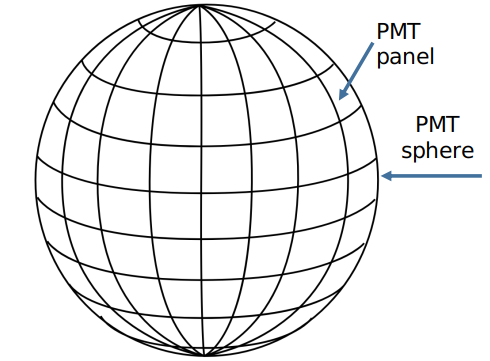
\includegraphics[width=5cm]{GroupPMTs.png}
	\caption{Group the PMTs by dividing the PMT sphere with latitudes and longitudes.}
	\label{GroupPMTs}
\end{figure}

For each panel, the selector first drops the PMTs triggered too early ($t_\mathrm{PMT}<100~ns$, where $100~ns$ is set as a default threshold). These PMTs could be triggered by noises, such as pre-pulsing. In the rest of the PMTs, the selector picks up one PMT with the earliest $t_\mathrm{PMT}$ in each panel. Thus the number of the PMTs is reduced to $n\times n$ for the fitter, i.e., $n_{select}=n\times n$. If $N\leq n_{select}$, the selector does nothing. 

We can also use the other timing parameter, such as the $t_{mode}$ or the $t_{median}$ for selecting the PMT in each panel. However, tests from the simulations for the scintillator phase show that using the earliest hit time gives less fit biases and better fit resolutions.
\end{itemize}